\input{settings}
\setlength{\emergencystretch}{2em}
\titleformat{\section}
  {\small\bfseries\raggedright}
  {}{0em}
  {}
  [{\color{WHU_Blue}\titlerule}]
\titlespacing*{\section}{0cm}{0.85em}{0.60em}
\titlespacing*{\subsection}{0cm}{0.50em}{0.30em}
\setlist[itemize]{topsep=0.20em, itemsep=0.20em, parsep=0em, partopsep=0em, leftmargin=1.25em}
\setlist[enumerate]{topsep=0.20em, itemsep=0.20em, parsep=0em, partopsep=0em, leftmargin=1.35em}
\renewcommand{\arraystretch}{0.98}
\renewcommand{\CJKglue}{\hskip 0.018em}

% 个人信息
%  cd C:\Users\31087\Documents\Obsidian_Vault\Resume\template
%  xelatex main_algo.tex
\newcommand{\school}{江南大学 · 控制科学与工程}

\newcommand{\resumeDecor}{
    \begin{tikzpicture}[remember picture, overlay]
        \node[anchor=north, inner sep=0pt](header) at (current page.north){
            
\includegraphics[width=\paperwidth]{images/header.png}
        };
        \node[anchor=west](school_logo) at (header.west){
            \hspace{0.5cm}
            
\includegraphics[width=0.15\textwidth]{images/whu_logo_1.png}
        };
        \node[anchor=east](school_name) at(header.east){
            \textcolor{white}{\textbf{\school}}
            \hspace{0.5cm}
        };
    \end{tikzpicture}

    \begin{tikzpicture}[remember picture, overlay]
        \node[opacity=0.05] at(current page.center){
            
\includegraphics[width=0.68\paperwidth, keepaspectratio]{images/whu_logo_big.png}
        };
    \end{tikzpicture}
}

\newcommand{\sectionIcon}[2]{\makebox[\widthof{#1}][c]{\color{WHU_Blue}{#1}}\quad #2}

%%%%%%%%%%%%%%%%%%%%
% 简历正文
%%%%%%%%%%%%%%%%%%%%
\begin{document}
\resumeDecor
\vspace*{-3.15em}
\scriptsize
\linespread{1.10}\selectfont

% 个人信息
\begin{minipage}{0.80\textwidth}
    \section[个人信息]{\sectionIcon{\faAddressCard}{个人信息}}
    \footnotesize
    \begin{tabularx}{\linewidth}{p{\widthof{求职意向:}}Xp{\widthof{最高学历:}}X}
        姓\ \ \ \ \ \ \ \ 名: & 梁邦一 &
        性\ \ \ \ \ \ \ \ 别: & 男 \\
        邮\ \ \ \ \ \ \ \ 箱: & yuejinai55@gmail.com &
        电\ \ \ \ \ \ \ \ 话: & +86 15515602693 \\
        英语等级: & CET-6 &
        求职意向: & 算法研发（视觉方向） \\
    \end{tabularx}
\end{minipage}
\hfill
\begin{minipage}{0.11\textwidth}
    \vspace{2.0em}
    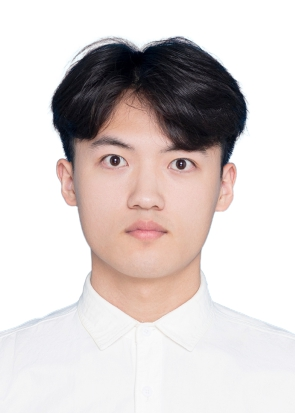
\includegraphics[width=\linewidth]{images/avatar.png}
\end{minipage}
\vspace{-0.60em}

\section[教育背景]{\sectionIcon{\faGraduationCap}{教育背景}}
\begin{itemize}
    \item {\textbf{控制科学与工程硕士，江南大学}}（\hl{中国科学院沈阳自动化研究所 · 机器人与智能系统全国重点实验室联合培养}） \hfill {2024.06--2027.06}
    \item {\textbf{自动化学士，郑州轻工业大学}} \hfill {2020.09--2024.06}
\end{itemize}

% 荣誉与组织经历
\section[荣誉与组织经历]{\sectionIcon{\faStar}{荣誉与组织经历}}
\begin{itemize}
    \item \textbf{中国机器人大赛暨 RoboCup 机器人世界杯中国赛} \hl{国家三等奖}（本科期间，参与机器人竞赛全流程）；校一等奖学金（2025.10、2026）；优秀毕业生（2024.06）；优秀班干部（2022.10）。
    \item 曾任本科班长、硕士党支部书记，具备需求收集、任务拆解、协同沟通与事项推进能力。
\end{itemize}

% 专业技能
\section[专业技能]{\sectionIcon{\faWrench}{专业技能}}
\begin{itemize}
    \item \textbf{视觉算法}：YOLO11s-seg、Ultralytics YOLO、Grounding DINO、Qwen3-VL、视觉 Embedding 检索、目标检测、实例分割、分类、连续值回归。
    \item \textbf{深度学习}：PyTorch、Transformer、CNN、Conformer、LLaMA-Factory、GRPO、4 机 8 卡 H20 多机多卡训练、bad case 归因与精度回归。
    \item \textbf{端侧部署}：TensorRT、ONNX、NVIDIA Jetson AGX Orin、模型量化与算子优化。
    \item \textbf{数据与评估}：数据集构建、类别一致性检查、训练/验证/测试集划分、标注质检、Corner Case 数据合成、标签库建设、验收准确率与误检漏检评估。
    \item \textbf{工程环境}：Python、C++、Linux / Ubuntu、Git、bash、ROS2、Docker、分布式训练配置、实验记录与复现。
\end{itemize}

% 实习经历
\section[实习经历]{\sectionIcon{\faBriefcase}{实习经历}}
{\small\textbf{CARIZON（大众×地平线合资智驾）}}\quad 感知数据部门算法实习生 \hfill {2026.06--至今}\\
{\scriptsize\color{WHU_Blue} 视觉识别算法 / 前沿算法组合落地 / 大模型后训练与评估}
\begin{itemize}
    \item 面向自动驾驶户外场景（红绿灯、交通标识、车辆、行人、锥桶等），采用 \textbf{Grounding DINO 开放词汇检测 + 专用 VLM 细粒度属性识别 + 视觉 Embedding 检索}的组合方案，实现\hl{目标定位与细粒度属性识别一体化}，服务长尾样本挖掘、Corner Case 筛选、标签校验与标签库建设。
    \item 融合车载多路传感器数据与回灌数据设计规则化 Tagger 与合成 pipeline：在 3W 条路口数据中筛选 3K 条转向 CLIP，\hl{标签验收准确率达 90\%、挖掘召回提升 10\%}；针对实车难覆盖的地面箭头、引导线等 Corner Case 用规则渲染 + 生成模型合成 5K 张训练样本，支撑挖掘模型冷启动迭代。
    \item 负责泊车障碍物识别 VLM 优化：筛选 1.8 万张挡轮杆图像完成数据清洗、标注校验与 Prompt 迭代；基于 \textbf{Qwen3-VL-8B + LLaMA-Factory} 在 \hl{4 机 8 卡 H20 集群完成全参数 SFT}；针对类别误判、高度不足等验收问题，设计\hl{基于 GRPO 的三元组策略优化方法}（1K 组"查询图—正样本—负样本"后训练数据），完成模型二次精标业务交付；同步梳理 mining-system 调用链，支撑模型迭代与问题排查。
\end{itemize}

\vspace{0.30em}
{\small\textbf{优奇智能科技有限公司（优必选子公司）}}\quad 人形机器人感知算法实习生 \hfill {2026.02--2026.05} \\
{\scriptsize\color{WHU_Blue} 目标检测与实例分割 / 模型评估与 bad case 归因闭环}
\begin{itemize}
    \item 负责 R11 接待机器人感知模型在 \textbf{NVIDIA Jetson AGX Orin} 端侧计算平台的部署：围绕 \textbf{TensorRT} 推理引擎完成 PyTorch $\rightarrow$ ONNX $\rightarrow$ TensorRT 模型转换、量化与算子性能优化，\hl{推理延迟降低 20\%}，在真机跑通检测/分割实时推理链路，形成\hl{“训练—部署—实机验证”端到端工程闭环}。
    \item 参与 R11 接待机器人感知模块 \textbf{YOLO11s-seg} 模型训练，基于 Python / PyTorch / Ultralytics YOLO 在 Ubuntu 环境完成实验环境搭建、数据配置、训练参数调整与基础效果验证，跑通\hl{目标检测 + 实例分割实验链路}，形成可复用训练配置与实验记录。
    \item 负责多场景视觉数据清洗、类别一致性检查、标注质检及\textbf{训练/验证/测试集划分}；围绕误检、漏检与分割边界不稳定 bad case 归因，区分数据覆盖、标注质量与模型能力等原因，输出问题清单与定向补数建议，建立\hl{“模型评估 → 问题归因 → 数据改进”的迭代闭环}。
\end{itemize}

\vspace{0.04em}
\section[科研与项目经历]{\sectionIcon{\faFlask}{科研与项目经历}}
{\small\textbf{面向具身智能灵巧操作的肌电-力融合感知与灵巧手抓取控制系统（灵心巧手） · 负责人}} \hfill {2025.02--2026.02} \\
{\scriptsize\color{WHU_Blue} 多模态感知 / Transformer 与 Conformer 时序建模 / ROS2 与 MuJoCo 仿真}
\begin{itemize}
    \item 面向 Linker Hand G20 灵巧手，搭建视觉 + sEMG + 力/触觉 + MuJoCo 仿真的\hl{多模态融合实验系统}，完成 Delsys Trigno 与 Sensel 多通道同步采集、时间戳对齐、任务标注与实时可视化，形成可复现感知数据入口。
    \item 基于 PyTorch 开展 \textbf{Transformer / 轻量 Conformer} 时序建模，支持\hl{力等级分类 + 连续力值回归双任务}；设计视觉—仿真策略—sEMG—触觉分层感知控制链路，围绕 ROS2 Topic 抽象模块化接口，打通 Python 数据侧与 Web 实时看板，形成感知—决策—执行端到端方案并支持模块独立替换与真机—仿真联调。
    \item 在机器人与智能系统全国重点实验室（中国科学院沈阳自动化研究所）承担课题实验链路组织与训练环境保障：使用 ROS2（Python/C++）完成节点开发与真机联调，独立完成 \hl{Linux 服务器环境搭建与维护}，保障 PyTorch 模型训练与实验复现稳定运行；\hl{系统性梳理手势识别、人机交互与机器人感知方向英文文献}，归纳传感器方案、算法框架、数据集与应用场景，支撑综述论文写作与课题技术路线判断。
\end{itemize}

\section[论文与研究成果]{\sectionIcon{\faBook}{论文与研究成果}}
三篇工作构成\hl{「综述定路线 — 算法破难点 — 系统做闭环」}的完整研究链条：
\begin{itemize}
    \item \hl{已中（JCR 一区，中科院二区）}：Liang B., Li N., Li G., et al. Sensing Technologies for Hand Gesture Recognition in Human-Robot Interaction: A Review[J]. IEEE Sensors Journal, 2025, 26(2): 1501-1519. \textbf{综述}：梳理数据手套、视觉与肌电等手势感知路线，对比精度、侵入性与成本取舍，为感知方案选型提供依据。
    \item \hl{在修（JCR 一区，中科院二区 Top）}：sEMG Conformer: Synergizing Local-Global Spatiotemporal Features for Continuous Force Estimation. Biomedical Signal Processing and Control. \textbf{算法核心}：卷积局部感受野 + 自注意力全局建模，解码肌电—指尖力映射，单模型支持力等级分类与连续力值回归。
    \item \hl{在投（JCR 一区，中科院二区）}：Dexterous Hand Grasping Control Based on Multimodal Sensory Fusion and Simulation Reinforcement Learning. \textbf{系统闭环}：MuJoCo 仿真强化生成抓取姿态，融合视觉、肌电与触觉构建分层控制链路，G20 上完成闭环部署验证。
\end{itemize}

\end{document}
